%% LyX 2.3.6.2 created this file.  For more info, see http://www.lyx.org/.
%% Do not edit unless you really know what you are doing.
\documentclass[english]{article}
\usepackage[T1]{fontenc}
\usepackage[latin9]{inputenc}
\pagestyle{plain}
\setcounter{secnumdepth}{0}
\usepackage{float}
\usepackage{amsmath}
\usepackage{amssymb}
\usepackage{graphicx}

\makeatletter
%%%%%%%%%%%%%%%%%%%%%%%%%%%%%% User specified LaTeX commands.


%%%%%%%%%%%%%%%%%%%%%%%%%%%%%%%%%%%%%%%%%%%%%%%%%%%%%%%%%%%%%%%%%%%%%%%%%%%%%%%%%%%%%%%%%%%%%%%%%%%%%%%%%%%%%%%%%%%%%%%%%%%%%%%%%%%%%%%%%%%%%%%%%%%%%%%%%%%%%%%%%%%%%%%%%%%%%%%%%%%%%%%%%%%%%%%%%%%%%%%%%%%%%%%%%%%%%%%%%%%%%%%%%%%%%%%%%%%%%%%%%%%%%%%%%%%%
\usepackage{amsfonts}

\setcounter{MaxMatrixCols}{10}
%TCIDATA{TCIstyle=LaTeX article (bright).cst}

%TCIDATA{OutputFilter=LATEX.DLL}
%TCIDATA{Version=5.00.0.2606}
%TCIDATA{<META NAME="SaveForMode" CONTENT="1">}
%TCIDATA{BibliographyScheme=Manual}
%TCIDATA{Created=Thursday, September 13, 2001 12:48:34}
%TCIDATA{LastRevised=Friday, February 24, 2006 07:54:08}
%TCIDATA{<META NAME="GraphicsSave" CONTENT="32">}
%TCIDATA{<META NAME="DocumentShell" CONTENT="Exams and Syllabi\SW\Assignment">}
%TCIDATA{Language=American English}

\setlength{\topmargin}{-1.0in}
\setlength{\textheight}{9.25in}
\setlength{\oddsidemargin}{0.0in}
\setlength{\evensidemargin}{0.0in}
\setlength{\textwidth}{6.5in}
\def\labelenumi{\arabic{enumi}.}
\def\theenumi{\arabic{enumi}}
\def\labelenumii{(\alph{enumii})}
\def\theenumii{\alph{enumii}}
\def\p@enumii{\theenumi.}
\def\labelenumiii{\arabic{enumiii}.}
\def\theenumiii{\arabic{enumiii}}
\def\p@enumiii{(\theenumi)(\theenumii)}
\def\labelenumiv{\arabic{enumiv}.}
\def\theenumiv{\arabic{enumiv}}
\def\p@enumiv{\p@enumiii.\theenumiii}


\parindent=0pt

\makeatother

\usepackage{babel}
\begin{document}
\begin{center}
\textbf{151-0530-00L, Spring, 2022}
\par\end{center}

\begin{center}
\textbf{Nonlinear Dynamics and Chaos II}
\par\end{center}

\begin{center}
\textbf{Homework Assignment 2}
\par\end{center}

\begin{center}
Due: Monday, April 11\\
Please email PDF file to Dr. Mattia Cenedese <mattiac@ethz.ch>
\par\end{center}

\bigskip{}

\begin{enumerate}
\item Derive the Hamiltonian equations of motion for a the coupled pendulums
shown in Fig. \ref{fig:coupled_pendula}. (The two point masses $m$
are placed at the tips of two massless rods of length $L$. Both joints
are frictionless; the constant of gravity is $g$.)
\begin{figure}[H]
\begin{centering}
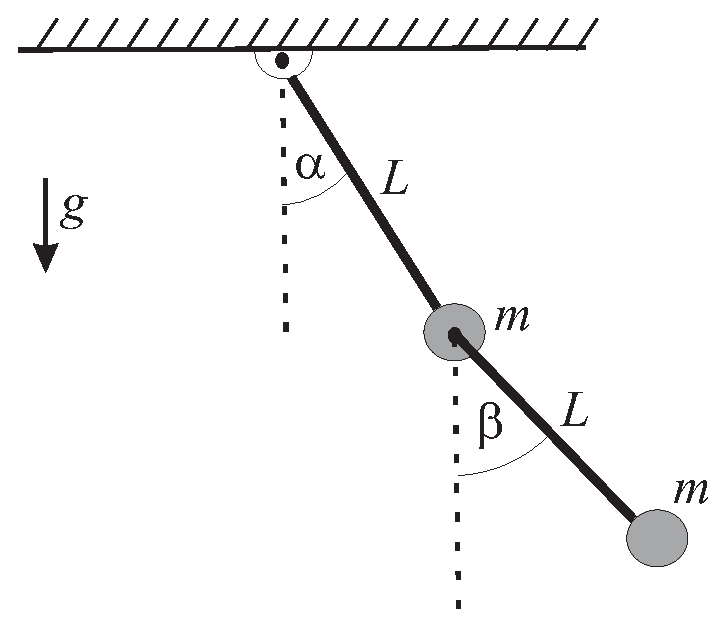
\includegraphics[width=0.4\textwidth,bb = 0 0 200 100, draft, type=eps]{../2.Homework and exam/coupledpendula.eps}\caption{Coupled system of two pendulums \label{fig:coupled_pendula}}
\par\end{centering}
\end{figure}
\item Consider the Lotka\textendash Volterra model
\begin{eqnarray}
\dot{h} & = & a_{1}h\left(1-bp\right),\label{1}\\
\dot{p} & = & -a_{2}p\left(1-ch\right),\nonumber 
\end{eqnarray}
for the interaction of a predator and a prey population. Here $h(t)$
and $p(t)$ denote the predator and prey populations, respectively,
as a function of time; $a_{1},a_{2},b,$ and $c$ are positive parameters.

(a) Show that system (\ref{1}) is Hamiltonian for $h,p>0$ after
an appropriate rescaling of time. Find the Hamiltonian. (Hint: Rewrite
(\ref{1}) as $\dot{h}=A(h,p)C(p),$ $\dot{p}=A(h,p)D(h)$ by defining
the functions $A,C$ and $D$ appropriately.)

(b)\ Using the Hamiltonian, argue that the two species can exhibit
stable coexistence, i.e., the system admits a stable fixed point.
(Hint: establish \emph{full nonlinear stability }for the fixed point).
\item Consider a two-dimensional steady \emph{compressible} fluid flow with
velocity field $\mathbf{v(x})=\left(u(x,y),v(x,y)\right)$, where
$\mathbf{x}=\left(x,y\right)$. Assume that the flow conserves mass,
i.e., its density function $\rho\left(\mathbf{x}\right)>0$ satisfies
the equation of continuity. The latter equation, in its general form
for unsteady flows, reads 
\[
\rho_{t}+\nabla\cdot\left(\rho\mathbf{v}\right)=0,
\]
valid or general, unsteady flow. Show that the equation of fluid particle
motion becomes a canonical Hamiltonian system after a rescaling of
time.
\item Consider a dynamical system defined on the two-dimensional torus $\mathbb{T}^{2}=S^{1}\times S^{1}.$
Such systems admit the general form
\begin{eqnarray}
\dot{\phi}_{1} & = & a(\phi_{1},\phi_{2}),\nonumber \\
\dot{\phi}_{2} & = & b(\phi_{1},\phi_{2}),\label{2}
\end{eqnarray}
where $\phi_{i}\in S^{1}$.

(a) Show that a physical example of system (\ref{2}) is found in
the motion of two uncoupled linear undamped oscillators. Specifically,
show that orbits of 
\begin{eqnarray*}
\ddot{x}+x & = & 0,\\
\ddot{y}+y & = & 0,
\end{eqnarray*}
are confined to two-dimensional invariant tori of the phase space.

(b) Assume that system (\ref{2}) has no fixed point (which is the
case in the oscillator example). Argue that (\ref{2}) then \emph{cannot}
be Hamiltonian, even after a rescaling of time. (\emph{Hint:} Use
the fact that a continuous function defined on a compact set must
have a minimum and a maximum). 
\item Show that for any dynamical system $\dot{q}=f(q,t)$, $q\in\mathbb{R}^{n}$,
one can select a canonically conjugate variable $p\in\mathbb{R}^{n}$,
such that the evolution of $(q(t),p(t))$ is governed by a Hamiltonian
system. (Thus any type of dynamics can be viewed as a projection from
a higher-dimensional Hamiltonian dynamical system.)
\end{enumerate}

\end{document}
